\chapter{Technique}

In this chapter, we will discuss the advantages and the limitations of combining symbolic execution with a debugger and, more in general, with any forms of concrete execution.

\section{Debuggers}

A {\em debugger}, according to \cite{PMA}, is a piece of software or hardware used to test or examine the execution of another program.
It is mainly designed to allow a developer to examine and control the internal state and the execution flow of a program.

Inspecting and also manipulating the execution context (the memory and the registers) of the program at any time is a fundamental operation during the reverse engineering process.

There are two types of debuggers from a user point of view:
\begin{itemize}
\item source-level, that allows the user to inspect the program state in terms of the source code when available;
\item low-level, with which the user operates only on disassembly;
\end{itemize}

Reverse engineering a software is a process that does not involve often the source code so low-level debuggers are the most used.

The main features of a debugger are the following:

\begin{itemize}
\item Single stepping: execute an instruction and return the control to the debugger;
\item Set a breakpoint: mark a place in the code or define a condition for which the execution is stopped so that the user can inspect the program state;
\item Modify execution: for example, change the value of a memory location to understand how a function works with a determinate input;
\item Hook exceptions: return the control to the debugger when an error like SEGFAULT occurs;
\end{itemize}

\section{Motivation}

The work of a reverse engineer is not simply reading assembly, often the code is hidden or very difficult to read and only with an automatic tool it can be understood.
A reverser makes an heavy usage of the debugger and in many cases the difficult code is revealed only during execution, the simplest example is a packed executable.

In a lot of malware samples, a target point in the program can be reached only under complex conditions, like in a malware with evasion techniques, and the program state can be very complex.

If we start symbolic execution from the entry point of the program the exploration may never reach the target point due to the limitations exposed in the previous chapter.
Even if that point is reached the path constraints and the symbolic expressions can be very complex and the exploration of the interesting code that follows the target point can be very expensive due to the time spent by the SMT solver to verify these complex expressions.

On the other hand, we would like to start the exploration directly from the beginning of the interesting code to avoid these issues. To this end we have to create a state from which to start the symbolic execution in a consistent way, setting the variables in the symbolic executor environment that are required for the correct behavior of the code that must be explored.
When done manually, this task can be time-consuming and error-prone.

However, the initial state for the symbolic execution may be created automatically by importing the concrete state from a concrete execution.

Since we do not know a priori which variables are involved during the execution of the code we need to take the entire concrete state and transfer it to the symbolic executor.

In this thesis, we propose to use a debugger to make easy for an analyst to reach the useful point.

This is the essence of our technique, transfer (even complex) states from a debugger to a symbolic executor and write back the results in order to synchronize both states. This makes possible for the reverser to continue the debugging after the exploration.

This technique can be very effective if there is the need to do symbolic execution of small pieces of code often during the debugging, so you can manually control the execution and solve difficult code in a surgical way.

Obviously, this approach is not limited to debuggers but can be extended to transfer the state from memory dumps, emulators or from a concrete execution controlled by a DBI framework\footnote{Dynamic Binary Instrumentation \cite{Net:phd2004}: a dynamic analysis technique that inserts analysis code at run-time in the "instrumented" program.} like Intel Pin \cite{Pin} or Frida \cite{Frida}.
%I this thesis we will cover the implementation of the technique in two popular debuggers.%, but in the future, I will integrate this also with a DBI framework.

\section{Description}
\label{descr}

If we try to imagine the simplest implementation of state transfer from a paused debugger to a symbolic executor it will be a simple copy of registers and memory.
However, this approach comes with severe disadvantages.

The address space of a process may be large thus copying all the memory is not practicable because of the slowness of the process. The memory must be requested to the debugger lazily.

%Another specific challenge is to avoid execution of large library code, but this depends on the design of the symbolic executor and we will discuss it in the implementation chapter.

Before the state transfer, the analyst must set the symbolic variables and its constraints. The constraints are required in order to force the symbolic executor to explore only the paths that can be executed starting from the current debugger state.
These constraints must not conflict with the required constraints that allow reaching of the concrete state that we are going to transfer. Since there is no previous symbolic exploration that collects these constraints this process requires an accurate analysis and a correct reverse engineering of the code executed before starting the state transfer. An error during this passage may compromise exploration and lead to unfeasible executions.

For example if we must set as symbolic a string read during the debugging with \verb|scanf("%s"...)| and we do not set also the constraints that it cannot contain whitespace characters, after the exploration the concretized string can contain whitespaces making it an input that can never be entered by the user.

In addition, a program state is not only registers and memory but also how the process interacted/must interact with the environment.
Environment synchronization is a challenging problem.

To do this we must build a mechanism to create a symbolic executor environment as similar as possible to the concrete environment. An example is synchronizing the position of the cursor associated with the opened file descriptors. In this thesis, we propose to interact with the environment saving the context of the concrete process, executing syscalls concretely and retrieve information from the operating system and then restoring the context just before the state transfer.

The reverse process, transfer the state found after the exploration to the debugger is not trivial. All the modification to the environment must be tracked and reproduced on the concrete environment, so the most reasonable way is to concretize the variables that we chose as symbolic input before the symbolic exploration, inject them in the debugger and run the paused process replicating the execution of the path found during the symbolic exploration.

\begin{figure}[H]
  \caption{High-level flow of the technique.}
  \centering
  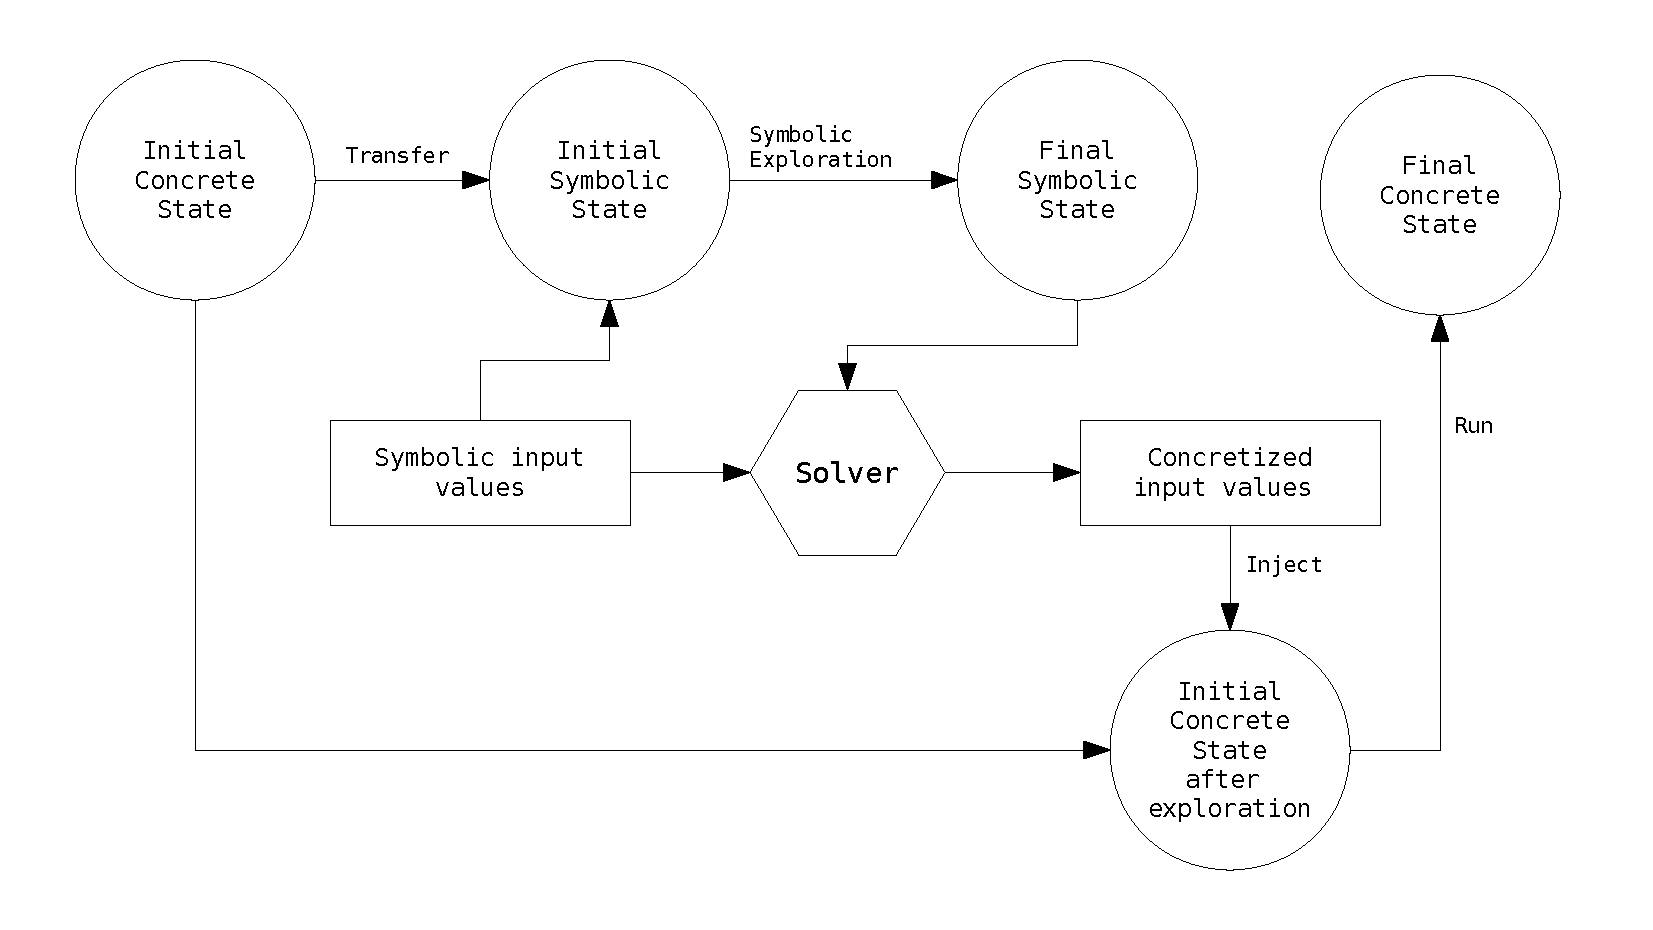
\includegraphics[width=1\textwidth]{g}
  \label{fig:g}
\end{figure}

\subsection{Memory Transfer Strategies}

During the development of the technique we identified three different strategies for handling the retrieving of the memory from the concrete process:

\begin{enumerate}  
\item Transfer the entire process memory during state creation;
\item Lazy transfer of pages when requested;
\item Lazy transfer of bytes when requested;
\end{enumerate}

The first is a bad choice, as motivated in section \ref{descr}, since the process memory is huge and a state transfer can consume too much time and memory.
The other two are reasonable strategies and in this thesis, we have chosen the last one after a preliminary experimental evaluation that showed how moving even single pages in place of just a few bytes can add a significant overhead.

%\section{Differencies with Dynamic Symbolic Execution}

%The main difference between our technique and DSE is that we do not drive the symbolic exploration using concrete inputs.
%The concrete process, paused using the debugger, is the data backend behind the symbolic executor.
%At the end of the exploration, if the target is reached the symbolic input is concretized using the collected constraints and injected into the process.% only if needed.

%The aims of these methods are totally different. DSE is used to improve symbolic execution, on the other hand, our approach is used to get the needed prerequisites (the initial state) to execute symbolically a piece of code from a complex environment.

%The two techniques are independent and can live alongside.

\section{Limitations}

A limitation of this approach is handling the process state in the operating system. In this section, we consider only the GNU/Linux operating system but the exposed concepts are the same for all operating systems.

A very important part of the environment is the metadata associated with a process in the operating system: the {\em Process Control Block}.

This record cannot be accessed from userspace and a synchronization tool working at user level, as in our design, cannot transfer information contained in that record to the symbolic executor environment. The information that is stored in the PCB is, for example, the opened file descriptors and their state, the stack canary, the brk value and so on. While some information in the PCB can be retrieved using syscalls, other kinds of information available in kernel space cannot be retrieved in a similar way, like seccomp filters\footnote{Seccomp filtering provides a means for a process to specify a filter for
incoming system calls.}.

When transferring the symbolic executor state to the debugger we cannot write these values in the debugged internal process space. Additionally, tracking all the side effects at user level may be extremely challenging and add a significant overhead.

Outside the userspace context, it is possible to have full access to the operating system using an emulator like QEMU \cite{qemu} to run the target program or using a hypervisor to access kernel memory.
Furthermore, for the user, kernel debugging is not a convenient task if he needs only to debug a user-space application. An error during kernel debugging leads to an operating system reboot, possibly wasting the time spent by the analyst.

Our technique cannot be used if the analyst does not know how the execution of the debugged process until the target point affected the variables that he wants to set as symbolic. As we said before a wrong constraints selection can lead to unfeasible executions and so the analyst is limited to use this technique only when he knows the behavior of the previously executed code.

The divergence between the symbolic execution and the concrete execution is a possible error, caused, for example, by the concretization of a symbolic value read from a file to a value that is not really in that file when we try to execute the found path in the debugger. A similar issue is present in DSE (section \ref{dynamic_limit}).
